\section{Introduction}


\subsection{Basic definitions}

\def\B{\mathscr{B}}
\def\Alg{\mathscr{A}}
\def\Mes{\mathscr{M}}
\def\Rajch{\mathscr{R}}
\def\W{\mathscr{W}}
\def\L{\mathscr{L}}
\def\T{\Hat T}
\def\CL{{\mathrm{CL}}}

\begin{frame}

    \frametitle{Chacon's automorphism}
    Let $h_1 = 1,\ h_{j+1} = 3h_j + 1$ be the sequence of heights.\\
    $h_j = \frac{3^j - 1}{2}$\\
    Chacon's automorphism $T$ is built via \textbf{cutting-and-stacking} procedure

  \begin{flushright}
  \includegraphics[height=40mm]{Ch3Sta.pdf}
  \end{flushright}
\end{frame}

\begin{frame}
    \frametitle{Generalized Chacon's automorphism}
    Similarly, we define generalized automorphism for arbitary p.\\
    Let $h_1 = 1,\ h_{j+1} = ph_j + 1$ be the sequence of heights.\\
    $h_j = \frac{p^j - 1}{2}$\\

  \begin{flushright}
  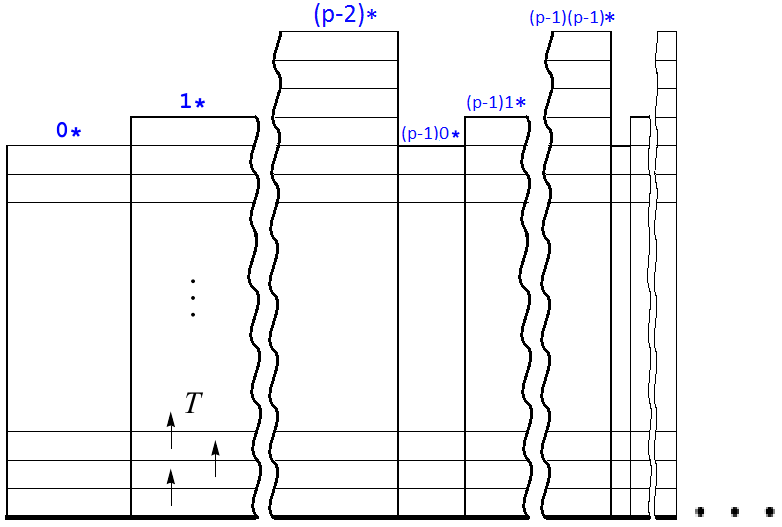
\includegraphics[height=45mm]{gen_stack.png}
  \end{flushright}
\end{frame}

\begin{frame}
    \frametitle{p-adic group}
    $\Gamma := \mathbb{Z}_p = \left\{x = \left(x_0, x_1, x_2, \ldots \right), x_k \in \{0, 1, \ldots, p - 1\} \right\}$\\
    $\lambda$ is the Haar measure on $\Gamma$. \\
    We define two $\lambda$-preserving transformations on $\Gamma$:\\
    \begin{itemize}
    \item $\sigma:\ x=\left(x_0, x_1, x_2, \ldots \right) \mapsto \sigma x = \left(x_1, x_2, \ldots \right)$
    \item $S:\ x \mapsto x + 1$, where $1:=(1,0,0,\ldots)$
    \end{itemize}
    Let $\phi: \Gamma \setminus \{(p-1,p-1,\ldots)\} \rightarrow \mathbb{Z}$ be the <<first not $(p-1)$>> functional:\\
    \[\phi(x):=x_i\text{ if }x=(p-1, \ldots, p-1, x_i, x_{i+1}, \ldots)\]
    \[\phi^{(0)}(x):=0;\ \phi^{(m)}(x):=\phi(x)+\phi(Sx)+\ldots+\phi(S^{m-1}x)\]
\end{frame}

\begin{frame}
    \frametitle{Chacon's automorphism on p-adic group}  
    $X_n := \left\{(x, i): x \in \Gamma, 0 \le i \le h_n - 1 + \phi(x)\right\}$\\    
    \[
        T_n(x, i):= \begin{cases} 
            (x, i+1) & \text{ if } i+1 \le h_n-1+\phi(x)\\
            (Sx, 0) & \text{ if } i = h_n - 1 + \phi(x)
            \end{cases}
    \]
    \[\psi: X_n \rightarrow X_{n+1},\ \psi_n(x, i) := (\sigma x, x_0 h_n + i + \mathbb{I}_{x_0 = p-1})\]
  \begin{center}
  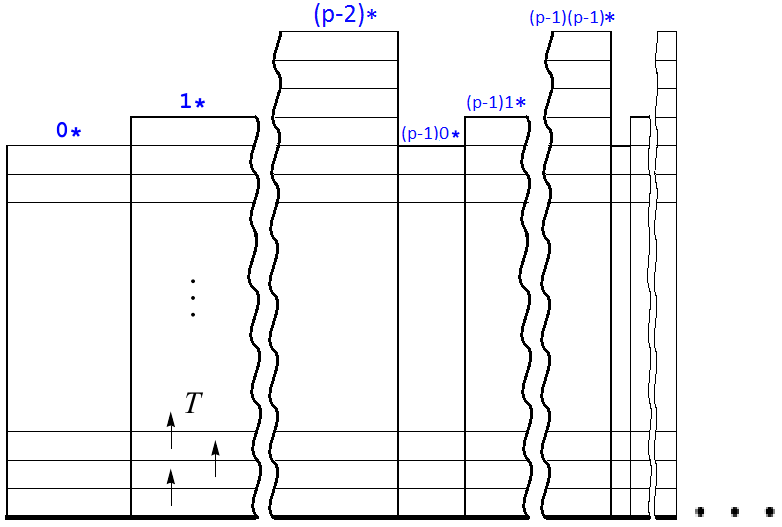
\includegraphics[height=35mm]{gen_stack.png}
  \end{center}
\end{frame}


\subsection{Polynomial constructions}


\begin{frame}


    \frametitle{Polynomial constructions}  
    \[\phi(x):=x_i\text{ if }x=(p-1, \ldots, p-1, x_i, x_{i+1}, \ldots)\]
    \[\phi^{(0)}(x):=0;\ \phi^{(m)}(x):=\phi(x)+\phi(Sx)+\ldots+\phi(S^{m-1}x)\]
    Let us define $\pi_m$ as the probability distribution of $\phi^{(m)}$ on $\mathbb{Z}$:
    \[\pi_m(j) = \lambda(\phi^{(m)}=j)\]
    We consider the sequences of polynomials $P_m^p$ produced by $\pi_m$ for fixed $p$ and $m$:
    \[P_m^p(t):= \mathbb{E}_\lambda\left[ t^{\phi^{(m)}(x)}\right] = \sum\limits_{j=0}^m \pi_m(j) t^j \]
\end{frame}


\subsection{Example}


\begin{frame}
  \frametitle{Results for p=3 }
  {\bf Theorem 1}\\(E.Janvresse, T. de la Rue, A.Prikhodko., V.Ryzhikov, '13).\\ \bigskip 
     For all $m \ge 0$, 
    \[P_{3m}(t)=t^m P_m^3(t)\ ;\]
    \[P_{3m+1}(t)=\frac{1}{3} t^m \left((1+t)P_m^3(t) + P_{m+1}^3(t) \right);\]
    \[P_{3m+2}(t)=\frac{1}{3} t^m \left(tP_m^3(t) + (1+t)P_{m+1}^3(t) \right);\]
      \begin{itemize}
   \item $P_m^3$ are palindromic
   \item Lee--Yang property: all roots of $P_m^3$ are real
   \item the family $P_m^3$ contains many irreducible polynomials
  \end{itemize}
 \end{frame}

\begin{frame}
  \frametitle{Results for p=3 }

  {\bf Theorem 2}\\ (E.Janvresse, T. de la Rue, A.Prikhodko., V.Ryzhikov, '13).\\ \bigskip 
    Let $T$ be the map associated with Chacon's substitution.\\

  $\Hat T^{mh_n} \wto P_m^3(\T)$ and the semigroup 
  $$
    \L = \overline{\{\T^k \where k \in \Set{Z}\}} = \{P_{m_1}^3(\T)\cdots P_{m_r}^3(\T)\T^s,\ \Theta\},
  $$
  where $\Theta$ is the orthoprojector to contants. \\
\end{frame}




\section{Polynomial constructions}


\subsection{Recurrent formulae}


\begin{frame}
    \frametitle{General result for arbitary p, m}
     {\bf Theorem.}\\ \bigskip
     For all $p \ge 3,\ m \ge 0$, $1 \le k \le p-1$:
     \bigskip 
     \begin{eqnarray*} 
     P_{pm}^p(t) & = &  t^{\Delta_{p-2} m}\ P_m^p(t)\ ; \\
     P_{pm+k}(t) & = &  \frac{1}{p} t^{\Delta_{p-2} m + \Delta_{k-1}}\sum\limits_{j=0}^{p-k-1} t^{jk} P_m^p(t) + \\
     & & + \frac{1}{p} t^{\Delta_{p-2} m + \Delta_{k-2}}\sum\limits_{j=0}^{k-1} t^{j(p-k)} P_{m+1}^p(t) 
      \end{eqnarray*}
     where $\Delta_n = \frac{n(n+1)}{2}$ is the $n$th triangle number\\
     (assuming $\Delta_{-1}=\Delta_0 = 1$)
\end{frame}


\subsection{Hypotheses}

\begin{frame}
    \frametitle{Hypotheses on $P_m^p(t)$}
  \begin{enumerate}
   \item $P_m^p$ are palindromic
   \item All roots of $P_m^p$ are on the unit circle
   \item the family $P_m^p$ contains irreducible polynomials
  \end{enumerate}
\end{frame}

\section{Palindromic property}
\subsection{Definitions}
\begin{frame}
    \frametitle{Definition of palindromic property}
    Recall: $\pi_m(j) = \lambda(\phi^{(m)}=j),P_m^p(t):= \mathbb{E}_\lambda\left[ t^{\phi^{(m)}(x)}\right] = \sum\limits_{j=0}^m \pi_m(j) t^j$
    
    Let $\phi_\star = \min\limits_x \phi(x), \phi^\star = \max\limits_x \phi(x), \delta=\phi^\star - \phi_\star$.
    
     Palindromic property: $\forall j,\ 0 \le j \le m\delta:   \pi_m(m\phi_\star + j)=\pi_m(m\phi^\star-j)$
     \center{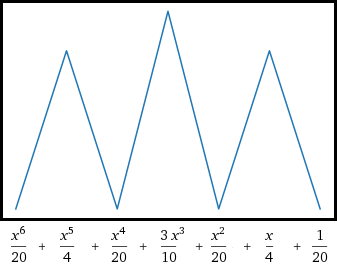
\includegraphics[scale=0.5]{palindromic}}
\end{frame}

\begin{frame}
    \frametitle{Generalization of $\phi$}
    We can generalize the definition of $\phi$ functional:
    $$
    \phi(x) = \begin{cases}
                    \omega(x_0), & 0 \le x_0 \le p - 2 \\
                    \phi(\sigma x), & x_0 = p - 1
                \end{cases}
    $$
    The classic case is hence described by $\omega(j)=j$.\\
    This is the only non-trivial $\omega$ for $p=3$.\\
    What are the conditions on $\omega$ implying to Palindromic property?
\end{frame}

\subsection{Theorem}
\begin{frame}
\frametitle{Antipalindromic functions}
We call a function $\omega$  \textit{antipalindromic} iff
\[\begin{cases}
	\mathrm{Ran }\ \omega = \{0,1, \ldots, \zeta\} \\
	\forall j,\ 0 \le j \le p-2: \  \omega(j) + \omega(p-2-j) = \zeta
\end{cases}\]
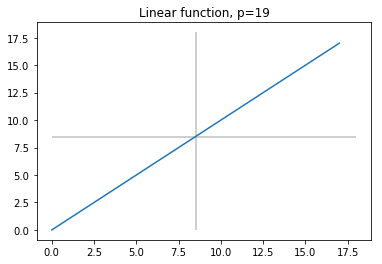
\includegraphics[width=0.5\linewidth]{linear}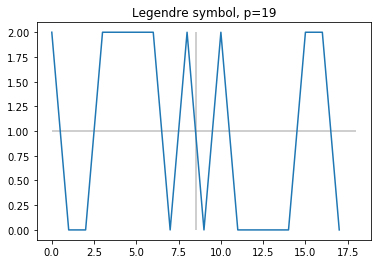
\includegraphics[width=0.5\linewidth]{legendre}
\end{frame}

\begin{frame}
\frametitle{Sufficient condition}
\textbf{Theorem.}
\begin{center}$\phi$ is palindromic $\iff$ $\omega$ is antipalindromic \end{center}
 
The statement follows from \textbf{Lemma:}
\begin{center}If $\omega$ is antipalindromic, $\{\phi(S^j x)\}_{j \ge 0} \overset{d}{=} \{ \zeta - \phi(S^{-j} x)\}_{j \ge 0}$\end{center}
\textbf{Inheritance of property.}
If $\omega$ gives a palindromic $\phi$, then $a\omega+b$ gives a palindromic $\phi$, too.
\end{frame}

\subsection{Examples}
\begin{frame}
\frametitle{First 5 polynomials for p=3,4,5}
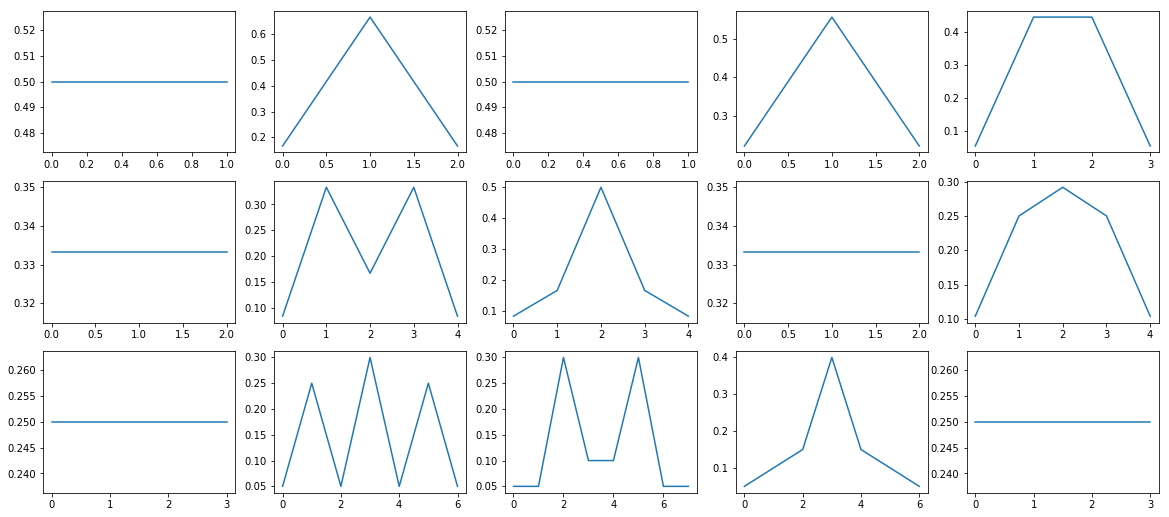
\includegraphics[width=\linewidth]{distributions}
\end{frame}

\section{Degrees of polynomials}
\subsection{Recurrence equations}
\begin{frame}
\frametitle{Degrees of polynomials}

\textbf{Polynomials}

\begin{align*} 
     P_{pm}^p(t) & =   t^{\Delta_{p-2} m}\ P_m^p(t)\ ; \\
     P_{pm+k}(t) & =   \frac{1}{p} t^{\Delta_{p-2} m + \Delta_{k-1}}\sum\limits_{j=0}^{p-k-1} t^{jk} P_m^p(t) + \\
     &  + \frac{1}{p} t^{\Delta_{p-2} m + \Delta_{k-2}}\sum\limits_{j=0}^{k-1} t^{j(p-k)} P_{m+1}^p(t) 
\end{align*}
\end{frame}

\begin{frame}
\frametitle{Degrees of polynomials}

\textbf{Degrees}
\begin{align*}
  d_{pm}^p &= m \Delta_{p-2} + d_m^p \\
  d_{pm+k}^p &= m \Delta_{p-2}+(p-k)(k-1)+\Delta_{k-2}+d_m^p+\\
   &+ \mathrm{max}\{p-k-1, s_m\},
\end{align*}
where $s_m = d_{m+1}^p-d_m^p$.

\begin{center}What is $\{s_m\}_{m \ge 0}$ like?\end{center}
\end{frame}

\subsection{Substitution sequence}
\begin{frame}
\frametitle{Structure of $s_m$}
Let $s_m = d_{m+1}^p-d_m^p$.\bigskip\\

 $\{s_m\}_{m \ge 0}$ is the \textbf{substitution sequence} generated by the rules:
\begin{itemize}
\item $j \in \left[0, \ldots, p-2 \right] \mapsto (p-2, p-1,\ldots,0)$, take $j$ twice
\item start with $(p-2)$
\item expand!
\end{itemize}
\end{frame}

\begin{frame}
\frametitle{Example}
Let $p=5$. What are the first terms of $\{s_m\}$?\bigskip\\

\begin{itemize}
\item $3 \mapsto 33210$
\item $2 \mapsto 32210$
\item $1 \mapsto 32110$
\item $0 \mapsto 32100$
\end{itemize}

We get $3 \mapsto 33210 \mapsto 33210\ 33210\ 32210\ 32110\ 32100 \mapsto \ldots$
\end{frame}

\subsection{Degrees}
\begin{frame}
\frametitle{Nice plots: $s_m$ and $d_m$, p=4}
\center
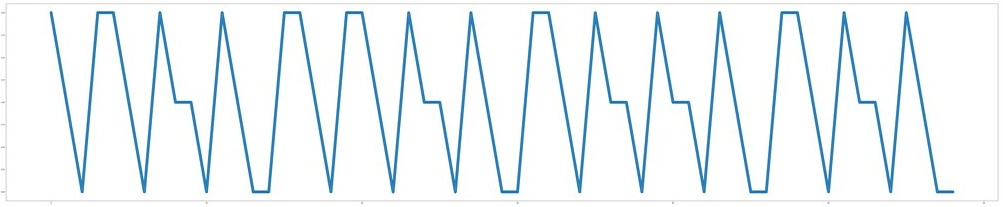
\includegraphics[width=0.9\linewidth]{s4}\\
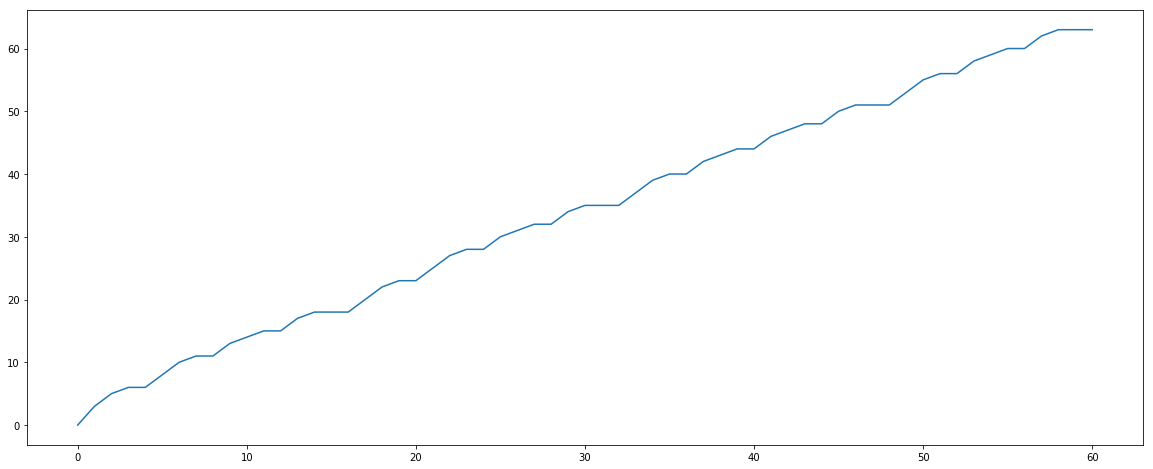
\includegraphics[width=0.9\linewidth]{degrees}
\end{frame}

\section{Conclusion}
\begin{frame}
\frametitle{Questions and hypotheses}
\begin{itemize}
\item Symmetrized polynomials $\tilde{P}_m^p(t)=t^{-d^p_m}P_m^p(t)$
\item Properties of $P_m^p$: roots, irreducibility
\item Weak limits of generalized automorphism
\end{itemize}
\end{frame}